\documentclass[a4paper, fontsize=11pt]{article}

\usepackage{amsmath,amsfonts,amsthm} % Math packages
\usepackage[english]{babel} % English language/hyphenation
%\usepackage{hyperref}
\usepackage{listings}
\usepackage{color}
\usepackage{verbatim}
\usepackage{graphicx}
\usepackage{booktabs}
\usepackage{float}


\usepackage[colorlinks=true,linkcolor=black,urlcolor=blue,
citecolor=blue]{hyperref}

%\bibliographystyle{ieeetr}
\bibliographystyle{apalike}

\definecolor{dkgreen}{rgb}{0,0.6,0}
\definecolor{gray}{rgb}{0.5,0.5,0.5}
\definecolor{mauve}{rgb}{0.58,0,0.82}


\lstset{frame=tb,
  language=C++,
  aboveskip=3mm,
  belowskip=3mm,
  showstringspaces=false,
  columns=flexible,
  basicstyle={\small\ttfamily},
  numbers=none,
  numberstyle=\tiny\color{gray},
  keywordstyle=\color{blue},
  commentstyle=\color{dkgreen},
  stringstyle=\color{mauve},
  breaklines=true,
  breakatwhitespace=true,
  tabsize=3
}

\begin{document}

\title{Project 2 FYS4150 \\ Eigenvalue problems}
\author{Audun Tahina Reitan and Marius Holm}

%----------------------------------------------------------------------------------------
%	PROBLEM 1
%----------------------------------------------------------------------------------------
\maketitle


\section{Abstract}



\section{Introduction}
In this project we'll develop code for solving eigenvalue problems. Our eigenvalue solver will be based on Jacobi's method, while the matrix we need to diagonalize is the tridiagonal Toeplitz matrix. This matrix has analytical eigenvalues and eigenvectors, which makes it easier for us to test our algorithms. 


\paragraph{}
The first problem we'll look at is the two-point boundary value problem of a buckling beam or a spring fastened at both ends. This problem has analytical solutions, and by adding a new variable along the diagonal we can study quantum mechanical problems. From quantum mechanics we will study the harmonic oscillator problem, with one or two electrons. For the two electron problem we can study the effects of Coulomb interaction and extract some interesting physics results.  The two electron problem even has analytical solutions for selected frequencies.\cite{PhysRevA.48.3561}

\paragraph{}
We introduce the relevant methods along with a brief explanation of our implementation.


Structure of report


\section{Methods}


\subsection{Eigenvalue problems}
Given the eigenvalue problem 

\begin{equation} \label{eigenvalue}
\textbf{A}\textbf{x}^{(v)}=\lambda^{(v)}\textbf{x}^{(v)}
\end{equation}

where \textbf{A} is a matrix of dimension $n$. We also have that $\lambda^{(v)}$ are the eigenvalues and $\textbf{x}^{(v)}$ the corresponding eigenvectors. From this we find that the eigenvalues of \textbf{A} are given by the $n$ roots of the characteristic polynomial given by:

\begin{equation}
P(\lambda)=\det(\lambda \textbf{I} - \textbf{A}) = \prod^{n}_{i=1}(\lambda_{i} - \lambda)
\end{equation}

This procedure is only valid for problems where we only need a small fraction of the eigenvalues and eigenvectors, or if the matrix is on a tridiagonal form. As our matrix is tridiagonal we can use the above procedure which leads us to the Jacobi method. A general procedure for solving equation \eqref{eigenvalue} is to perform similarity transformations until the original matrix \textbf{A} is either on diagonal form or is a tridiagonal matrix which then easily can be diagonalized. The general procedure leads to the well known Householder's algorithm.\cite{Jensen}


\subsection{Jacobi's method}
Given an $n \times n$ orthogonal transformation matrix

\begin{equation}
\textbf{S} =
\begin{pmatrix}
1 & 0 & \hdots & 0 & 0 & \hdots & 0 & 0 \\
0 & 1 & \hdots & 0 & 0 & \hdots & 0 & 0 \\
\hdots & \hdots & \hdots & \hdots & \hdots & \hdots & 0 & \hdots \\ 
0 & 0 & \hdots & \cos \theta & 0 & \hdots & 0 & \sin \theta \\
0 & 0 & \hdots & 0 & 1 & \hdots & 0 & 0 \\
\hdots & \hdots & \hdots & \hdots & \hdots & \hdots & 0 & \hdots \\
0 & 0 & \hdots & 0 & 0 & \hdots & 1 & 0 \\ 
0 & 0 & \hdots & \sin \theta & \hdots & \hdots & 0 & \cos \theta \\
\end{pmatrix}
\end{equation}

with the property $\textbf{S}^{\textbf{T}}=\textbf{S}^{-\textbf{1}}$. This matrix performs a plane rotation around an angle $\theta$ in the Euclidean $n$-dimensional space. Which means that the non-zero matrix elements are given by
\begin{equation}
s_{kk}=s_{ll}=\cos \theta, \:\: s_{kl}=-s_{lk}=-\sin \theta, \:\: s_{ii}=-s_{ii}=1 \quad i \neq k \: \: i \neq l,
\end{equation}

A similarity transformation 

\begin{equation}
\textbf{B}=\textbf{S}_{u\textbf{T}} \textbf{A} \textbf{S},
\end{equation}

results in 

\begin{flalign*}
b_{ii} &= a_{ii}, \: i \neq k, i\neq l 
\\
b_{ik} &= a_{ik} \cos \theta - a_{il} \sin \theta, \: i \neq k, i\neq l 
\\
b_{il} &= a_{il} \cos \theta + a_{ik} \sin \theta, \: i \neq k, i\neq l 
\\
b_{kk} &= a_{kk} \cos^{2} \theta - 2 a_{kl} \cos \theta \, \sin \theta + 		a_{ll} \sin^{2} \theta 
\\
b_{ll} &= a_{all} \cos^{2} \theta + 2 a_{kl} \cos \theta \, \sin \theta + 		a_{kk} \sin^{2} \theta 
\\
b_{kl} &= (a_{kk} - a_{ll}) \cos \theta \, \sin \theta + a_{kl} (\cos^{2} \theta - sin^{2} \theta)
\end{flalign*}

We can choose the angle $\theta$ as we wish, while making sure that all the non-diagonal matrix elements, $b_{kl}$ become zero. The algorithm which follows is then quite simple. We do a number of similarity transformations until the sum over the squared non-diagonal matrix elements are less than some chosen tolerance, typically less than $10^{-8}$. We therefore seek to minimize

\begin{equation}
\text{off}(\textbf{A}) = \sqrt{\sum^{n}_{i=1} \sum^{n}_{j=1, \: j \neq i} a_{ij}^{2}}
\end{equation}



\subsection{Scaling equations}
\paragraph{Transformation matrix}

For Jacobi's method the the rotational elements $\sin \theta = s$ and $\cos \theta = c$ with $\tan \theta = t = s / c$ is given by:

\begin{equation}
\cot 2\theta = \tau = \frac{a_{ll} - a_{kk}}{2 a_{kl}}
\end{equation}

\begin{equation}
\cot 2\theta = \frac{1}{2}\left(\cot \theta - \tan \theta \right) \implies t^2 + 2 \tau t - 1 = 0 \implies t = -\tau \pm \sqrt{1 + \tau^2} 
\end{equation}

\begin{equation}
c = \frac{1}{\sqrt{1+ t^2}}
\end{equation}

\begin{equation}
s = t\,c
\end{equation}

For $t$ we choose the solution to the 2nd degree formula that returns the smallest answer so that $t$ does not reach very high values. We do this because of the risk for loss of significance because of cancellation in the equation for $t$ when $\tau$ becomes so big that $\sqrt{1 + \tau^2} \approx \tau $.

\begin{equation}
t = \frac{1}{\tau + \sqrt{1 + \tau^2}}, \quad \tau > 0.0
\end{equation}

\begin{equation}
t = \frac{-1}{-\tau + \sqrt{1 + \tau^2}}, \quad \tau \leq 0.0
\end{equation}

These two solutions are equivalent to the smallest solution of the 2nd degree equation, and are numerical stable.

\paragraph{Quantum mechanics}
We are also interested in quantum mechanical problems where we want to solve the radial part of Schr\"{o}dinger's equation for one electron in a harmonic oscillator potential. The equation is given as:

\begin{equation}
-\dfrac{\hbar^2}{2m}\Big(\dfrac{1}{r^2} \dfrac{d}{dr} r^2 \dfrac{d}{dr} - \dfrac{l(l+1)}{r^2} \Big) R(r) +V(r)R(r)=E \, R(r)
\end{equation}

$V(r)$ for a harmonic oscillator potential is given as $V(r)=\frac{1}{2}kr^2$ with \\$k=m \omega^2$ and where $E$ is the energy of the harmonic oscillator in three dimensions. $\omega$ is the oscillator frequency, and the energies are given as:

\begin{equation}
E_{nl} = \hbar \omega \Big(2n+l+\frac{3}{2} \Big), \: \text{with} \: n=0,1,2, \hdots \: \text{and} \: l=0,1,2,\hdots
\end{equation}

Since we have made the transformation into spherical coordinates we have $r \in [0, \infty)$, and the quantum number $l$ is the orbital momentum of the electron. We then substitute $R(r)=\dfrac{1}{r}u(r)$ and get

\begin{equation}
\dfrac{\hbar^2}{2m} \dfrac{d^2}{dr^2} u(r) + \Big(V(r) + \dfrac{l(l+1)}{r^2} \dfrac{\hbar^2}{2m}\Big) u(r) = E \, u(r)
\end{equation}

With boundary conditions $u(0)=0$ and $u(\infty)=0$. We introduce the dimensionless variable $\rho = (1/\alpha)r$ where $\alpha$ is a constant with dimension length. We set $l=0$, and insert $V(\rho)=(1/2)k\alpha^2 \rho^2$. This gives us the following equation

\begin{equation}
-\dfrac{\hbar^2}{2m\alpha^2} \dfrac{d^2}{d\rho^2} \, u(\rho) + \dfrac{k}{2} \alpha^2 \rho^2 \, u(\rho) = E \, u(\rho) \quad |\cdot \dfrac{2m\alpha^2}{\hbar^2}
\end{equation}

\begin{equation}
-\dfrac{d^2}{d\rho^2} \, u(\rho) + \dfrac{mk}{\hbar^2} \alpha^4 \rho^2 \, u(\rho) = \dfrac{2m\alpha^2}{\hbar^2} E \, u(\rho) 
\end{equation}

Fixing the constant $\alpha$ as 

\begin{equation}
\alpha=\Big(\dfrac{\hbar^2}{mk}\Big)^{\frac{1}{4}}
\end{equation} 

We also define $\lambda=\dfrac{2m\alpha^2}{\hbar^2}E$ which lets us write the Schr\"{o}dinger equation as

\begin{equation}
-\dfrac{d^2}{d\rho^2}u(\rho) + \rho^2 \, u(\rho) = \lambda \, u(\rho)
\end{equation}

A lot of the same steps as above are repeated for the problem considering quantum dots in three dimensions with two electrons. I will therefore only state the final result along with the necessary constants that are defined. We then find the Schr\"{o}dinger equation as:

\begin{equation}
-\dfrac{d^2}{d\rho^2}\psi(\rho) + \omega^2_{r}\rho^2 \, u(\rho) + \frac{1}{\rho} = \lambda \, \psi(\rho)
\end{equation}

where we have defined  $\omega_{r}^2$ as

\begin{equation}
\omega^2_{r}=\dfrac{1}{4} \dfrac{mk}{\hbar^2} \alpha^4
\end{equation}

and fixing $\alpha$ by requiring 

\begin{equation}
\alpha = \dfrac{\hbar^2}{m\beta e^2}.
\end{equation}

Finally we have defined $\lambda$ as

\begin{equation}
\lambda=\dfrac{m\alpha^2}{\hbar^2}E
\end{equation}



\subsection{Implementation}

For the Jacobi's rotation method we implemented the algorithm given on page 217 in \cite{Jensen} and using the scaling and rewriting we have done the transformation matrix. In the github repository cited below the program can be found in the \verb+jacobi.cpp+ file. In order to find the highest valued off-diagonal element we took the upper triangular part of the matrix given, removed the diagonal, and then used Armadillos own methods to find the maximum absolute value element. For further details regarding implementation, see comments in the different programs.


\paragraph{}
All our code, calculations, unittests, and plots used can be found in \href{https://github.com/auduntre/FYS4150/tree/master/Project%202}{Auduns GitHub repository}.

\section{Results}
\subsection{Preservation of dot product}
We want to show that an orthogonal transformation preserves the dot product and orthogonality. Given a basis of vectors $\textbf{v}_{i}$

\begin{equation}
\textbf{v}_{i}=
\begin{bmatrix}
v_{i1} \\
v_{i2} \\
\vdots \\
v_{in}
\end{bmatrix}
\end{equation}

And assuming that the basis is orthogonal.

\begin{equation}
\textbf{v}^{T}_{j} \textbf{v}_{i} = \delta_{ij}
\end{equation}

The transformation is given by

\begin{equation}
\textbf{w}_{i} = \textbf{U} \textbf{v}_{i}
\end{equation}

As the transformation matrix \textbf{U} is orthogonal we have $\textbf{U}^{T}\textbf{U} = \textbf{I}$.

\begin{align*}
\textbf{w}_{i} \cdot \textbf{w}_{j} & =\textbf{U} \textbf{v}_{i} \cdot \textbf{U} \textbf{v}_{j} = (\textbf{U}\textbf{v}_{i})^{T}(\textbf{U}\textbf{v}_{j})=(\textbf{U}^{T} \textbf{v}_{i}^{T})(\textbf{U}\textbf{v}_{j})\\
&= \textbf{v}_{i}^{T} (\textbf{U}^{T} \textbf{U}) \textbf{v}_{j}= \textbf{v}_{i}^{T} \, \textbf{I} \, \textbf{v}_{j} =  \textbf{v}_{i}^{T} \,  \textbf{v}_{j} = \textbf{v}_{i} \cdot \textbf{v}_{j} = \textbf{v}^T_{i} \textbf{v}_{j}
\end{align*}

As $\textbf{w}_{i} \cdot \textbf{w}_{j} = \textbf{v}_{i} \cdot \textbf{v}_{j}$ the dot product is preserved. The same applies for $\textbf{v}_{i} \cdot \textbf{v}_{j} = \textbf{v}^T_{i} \textbf{v}_{j} = \delta_{ij}$ which implies that orthogonality is also preserved. This means that the Jacobi's rotational method which multiple orthogonal transfromations preserves the orthogonality and dot product of the columns in the system we trasnform.

\subsection{Eigenvalues of one electron in the harmonic oscillator}

Using one electron in the harmonic oscillator and solving using the Jacobi's method we get the following result on the apporixmation of the analytical eigenvalues $\lambda = 3, 7, 11, 15$ for the system, varying the number of integration points $N$:

\begin{table}[htp]
\begin{center}
\begin{tabular}{@{}llllllll@{}}
\toprule
     & \multicolumn{7}{c}{N}               \\ \cmidrule(l){2-8} 
Absolute error & 10 & 25 & 50 & 75 & 100 & 150 & 200 \\ \midrule
$|\lambda_1 - \hat{\lambda}_1|$    &    $8.05\mathrm{E}{-2}$&    $1.25\mathrm{E}{-2}$&    $3.13\mathrm{E}{-3}$&    $1.39\mathrm{E}{-3}$&     $7.81\mathrm{E}{-4}$&     $3.47\mathrm{E}{-4}$&      $1.95\mathrm{E}{-4}$\\
$|\lambda_2 - \hat{\lambda}_2|$    &    $4.16\mathrm{E}{-2}$&    $6.30\mathrm{E}{-2}$&    $1.57\mathrm{E}{-2}$&    $6.95\mathrm{E}{-3}$&     $3.91\mathrm{E}{-3}$&     $1.73\mathrm{E}{-3}$&      $9.74\mathrm{E}{-4}$\\
$|\lambda_3 - \hat{\lambda}_3|$    &    $1.06$&    $1.54\mathrm{E}{-1}$&    $3.81\mathrm{E}{-2}$&    $1.68\mathrm{E}{-2}$&     $9.34\mathrm{E}{-3}$&     $4.04\mathrm{E}{-3}$&     $2.18\mathrm{E}{-3}$\\
$|\lambda_4 - \hat{\lambda}_4|$    &    $2.08$&    $2.83\mathrm{E}{-1}$&    $6.54\mathrm{E}{-2}$&    $2.57\mathrm{E}{-2}$&     $1.18\mathrm{E}{-2}$&     $2.02\mathrm{E}{-3}$&     $1.42\mathrm{E}{-3}$\\ \bottomrule
\end{tabular}
\caption{Absolute error between the analytically known eigenvalues of the one-electron energies and our numerically calculated eigenvalues.}
\end{center}
\end{table}


\subsection{Quantum dots, plots}


\begin{figure}[H]
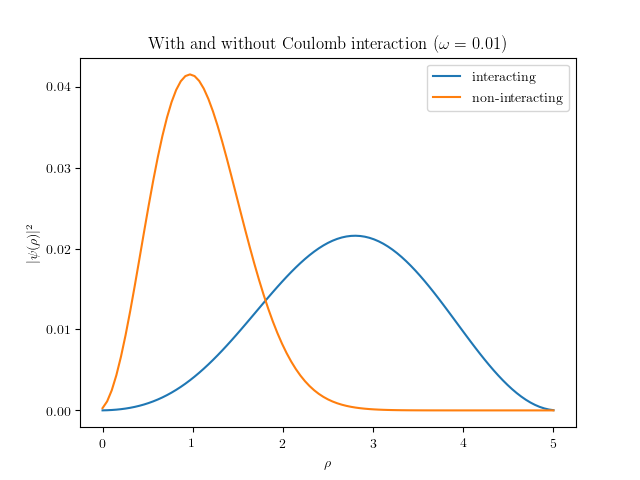
\includegraphics[scale=0.8]{interaction.png}
\caption{Comparing the energy levels for a system with and without Coulomb interation with $\omega_{r}=0.01$.}
\label{Coulomb}
\end{figure}


\begin{figure}
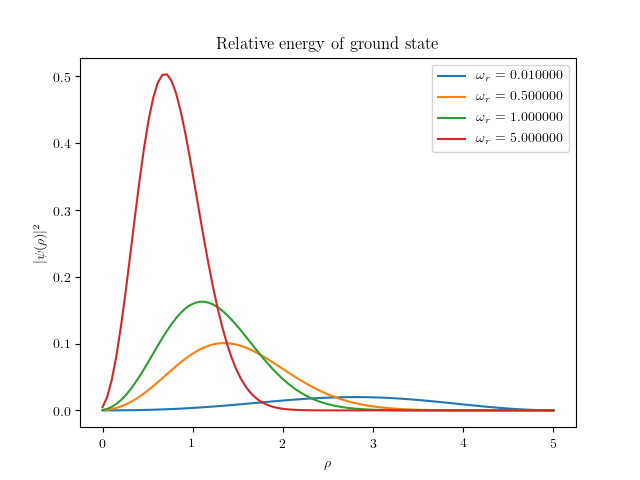
\includegraphics[scale=0.8]{twoelectrons.png}
\caption{Probability distribution for the ground state of a two-electron system including Coulomb interaction. Plotted for different values of $\omega_{r}$, where $\omega_{r}$ is a parameter which reflects the strength of the oscillator potential.}
\label{two-electron}
\end{figure}



\section{Discussion}
\subsection{Jacobi method}
The Jacobi method is generally a slower algorithm than those based tridiagonalization. However the Jacobi method is easy to parallelize which can improve performance significantly. The main reason for the Jacobi methods slow convergence is that for each new rotation, matrix elements which were zero might change to non-zero values.


\paragraph{}
For the case with one electron we would have needed to choose $N > 200$ in order to get numerical eigenvalues, $\hat{\lambda}_i$ that are able to reproduce the analytical ones, $\lambda_i$ with four leading digits after the decimal point (which means an absolute error $< 10^{-4}$). The Jacobi method is very slow for too large $N$ values, and doing the calculations with an $N > 200$ a modern laptop takes several minutes to complete the calculations. 

\paragraph{}
It would be of interest to investigate more effective methods like the Householder's method for large values of $N$, and see what differences a significant increase in integration points would result in.


\bibliography{references}
\end{document}